
\section{Thickness Evolution in Higher-Order Models}

\subsection{Conservation of mass}
For an ice sheet (or any depth-integrated mass flow), conservation of mass can be expressed by

\begin{align*}
\frac{\partial H}{\partial t}=-\nabla \cdot \left( UH \right)+\dot{b}
\end{align*}

The change in thickness per unit time is given by the negative of the flux divergence plus a source term. We can expand this a bit as,


\begin{align*}\frac{\partial H}{\partial t}=-\left( \frac{\partial \left( UH \right)}{\partial x}+\frac{\partial \left( VH \right)}{\partial y} \right)+\dot{b}, \\ 
\end{align*}

where $\vec{U}$ is the depth-averaged velocity vector (in map plane), and \textit{U} and \textit{V} are the depth integrated \textit{x} and \textit{y} velocity fields, \textit{H} is the ice thickness, and $\dot{b}$ is the source term, which is the surface mass balance (>0 for accumulation and <0 for ablation). Note that the negative sign in front of the divergence (terms in parentheses on the right-hand side) insures sensible behavior. Consider a section of the ice sheet where the thickness is nearly constant and there is no accumulation or ablation. If the velocity gradient along-flow is negative (the ice is slowing down), we expect that to lead to thickening locally (left-hand side of the equation > 0) and vice versa (if the ice is speeding up along flow, that should lead to thinning locally). This is the equation that needs to be solved to calculate ice sheet evolution.

\section{A diffusive approach}
For the case of a SIA model, the values of \textit{U} and \textit{V} are recast in terms of ice thickness and elevation gradients, in which case the whole problem can be recast as a diffusion equation in ice thickness. In 1d, the equation becomes

\begin{align*}
\frac{\partial H}{\partial t}=\frac{\partial }{\partial x}\left( D\frac{\partial h}{\partial x} \right)+\dot{b},\quad D=\frac{2A}{n=2}\left( \rho g \right)^{n}H^{n+2}\left| \frac{\partial h}{\partial x} \right|^{n-1},
\end{align*}

where \textit{D} is the non-linear diffusivity (because it depends on the solution to the equation, \textit{H}), \textit{A} is the rate factor in Glen's flow lay and \textit{n} is the power-law exponent, \textit{h} is the ice surface elevation, and \textit{\(\rho{}\)} and \textit{g} are the ice density and the acceleration due to gravity. Importantly, we need only local information in order to solve the above equation. If our velocity solution can not be solved locally, as in the case of higher-order models, we cannot easily use the above formulation to solve ice sheet evolution. In an attempt to use this form and retain a diffusion-solution approach to the problem (diffusion problems generally have nice numerical properties), we could try the following approach (again, in 1d only),

\begin{align*}
\frac{\partial H}{\partial t}=\frac{\partial }{\partial x}\left( D\frac{\partial h}{\partial x} \right)+\dot{b},\quad D=UH\left( \frac{\partial h}{\partial x} \right)^{-1},
\end{align*}

where the \textit{U} in the expression for \textit{D} is the depth-integrated velocity field from the higher-order model. This is the approach initially taken by \href{http://www.agu.org/journals/jb/jb0308/2002JB002329/}{Pattyn (2003)}. Notice, however, that ice sheet surface slope is in the denominator of the diffusivity here and, as the slopes get smaller and smaller, as they tend to do in regions of fast flow like ice streams and ice shelves, the diffusivity will get larger and larger (approaching infinity as the slope goes to zero). The faster velocities in these regions appear in the numerator of the diffusivity, also making it larger. This is a severe restriction on this approach because the diffusive CFL condition says that

\begin{align*}
\Delta t<\frac{\left( \Delta x \right)^{2}}{2D},
\end{align*}

where \textit{\(\Delta{}\)t} is the time step required for numerical stability and \textit{\(\Delta{}\)x} is the grid spacing. As the diffusivity goes to infinity (i.e., for faster flows and shallower slopes), the stable time step goes to zero. Thus in practice, this approach has proven very difficult to use for calculating ice sheet evolution in most of the areas we care about. An alternate approach is needed.

\subsection{Advection schemes}
An alternate approach is to solve the evolution equation using an advection scheme. Numerically, advection schemes can be more problematic than diffusion schemes, but in some cases like this one, they are difficult to avoid. The most general advection scheme is a first-order, upwind-advection scheme (first-order refers to first-order accurate), and we will outline the implementation of such a scheme below.

Most ice sheet models (and fluid dynamic models in general) perform calculations on a "staggered" grid of the type shown below, where velocity components live on one grid and scalar components (e.g. temperatures, pressures, thickness, etc.) live on a grid that is staggered by 1/2 grid space in the horizontal dimensions (this is essential for numerical reasons that we won't discuss here).

%\begin{figure}
%  \begin{center}
%    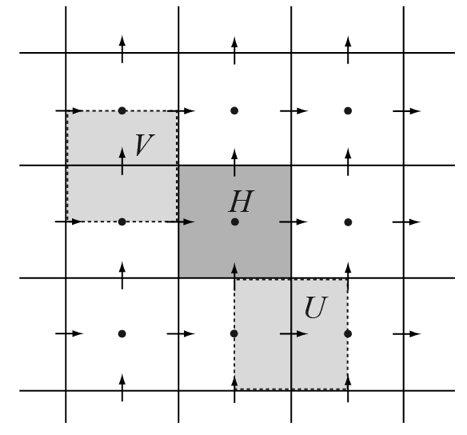
\includegraphics[width=0.9\columnwidth]{\dir/figs/Stag_grid.png}
%  \end{center}
%\caption{Staggered grid in two dimensions, showing scalars (like thickness, \textit{H}) at grid cell centers and velocity components, \textit{U} and \textit{V}, at grid cell faces. This is a "C" grid. Another staggered-grid possibility is a "B" grid, for which both velocity components live at the grid cell corners. While CISM uses a B grid, averaging of corner velocities to face centers allows one to express them on a C grid if necessary.}
%  \label{fig:stag_c_grid}
%\end{figure} 

A control volume (or finite volume) approach to solving the equation 

\begin{align*}
\frac{\partial H}{\partial t}=-\left( \frac{\partial \left( UH \right)}{\partial x}+\frac{\partial \left( VH \right)}{\partial y} \right)+\dot{b} \\ 
\end{align*}

would be to integrate our equation over a control volume centered on the scalar values (Figure \ref{fig:stag_C_grid}). Ignoring source terms for now, and assuming flow only along the \textit{x} direction only (that is, assuming that \textit{V}\(\sim\)0) we have

\begin{align*}
\frac{\partial H}{\partial t}=-\frac{1}{\Delta y\Delta x}\int_{s}^{n}{\int_{w}^{e}{\frac{\partial \left( UH \right)}{\partial x}}}dxdy=-\frac{1}{\Delta y\Delta x}\left( HU_{e}-HU_{w} \right)\Delta y. \\
\end{align*}

The "east" and "west" (subscripts \textit{e} and \textit{w}) faces of the control volume are shown in Figure \ref{fig:stag_C_grid2}.

%\begin{figure}
%  \begin{center}
%    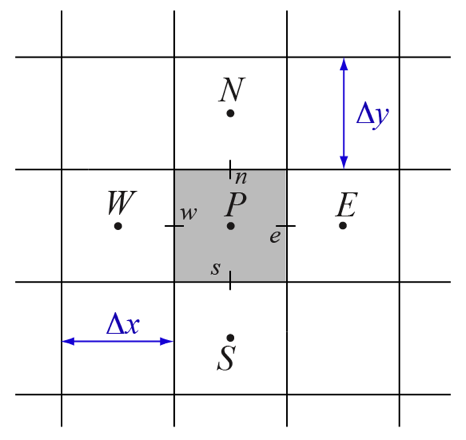
\includegraphics[width=0.9\columnwidth]{\dir/figs/Stag_gridb.png}
%  \end{center}
%  \caption{Staggered grid in two dimensions, showing locations of interfaces and control volume dimensions. Interfaces \textit{e}, \textit{w}, \textit{n} and \textit{s} connect the volume centered at \textit{P} with those volumes to the east, west, north, and south (\textit{E}, \textit{W}, \textit{N}, and \textit{S}).}
%  \label{fig:stag_c_grid2}
%\end{figure} 

In the above equation, we've deliberately left it vague as to which value of \textit{H} is being advected across the east and west interfaces, into or out of the volume. This is where the term "upwinding" comes in -- we choose the scalar value to advect across the interface based on an upwinding criterion. If, for example, the flow at interface \textit{e} is from left to right (\textit{U}>0), we would advect the value of \textit{H} at \textit{P} $out$ of the volume centered at \textit{P} and $into$ the volume centered at \textit{E}. If, on the other hand, the flow at \textit{e} was from right to left (\textit{U}<0), we would advect the value of \textit{H} at \textit{E} $into$ the volume at \textit{P} and $out$ of the volume at \textit{E}. 

The product of velocity, thickness, and the grid spacing at each interface gives a volume flux in units of cubic meters per year. The sum of the volume fluxes over the total number of faces being considered (two in this case, but four for the 2d case) gives the total volume flux in (total>0) or out (total<0) of the volume. When this number is divided by the area of the volume, the result is the mean thickness change in that volume per unit time required to maintain conservation of mass.

\subsection{Explicit vs. Implicit Evolution Schemes}
Is this an explicit or implicit scheme? If we discretize the right-hand side of the primary equation in time we get

\begin{align*}
  & \frac{\partial H}{\partial t}=-\nabla \cdot \left( UH \right)+\dot{b}, \\
 & \frac{H_{t=1}-H_{t=0}}{\Delta t}\approx -\nabla \cdot \left( UH \right)+\dot{b}.\\
\end{align*}

This can be rearranged to,

\begin{align*}
H_{t_{t=1}}\approx H_{t=0}+\left[ -\nabla \cdot \left( UH \right)+\dot{b} \right]_{t=0}\Delta t.
\end{align*}

The thickness at the new time step $t=1$ is a function of \textit{only} variables evaluated at the previous time step $t=0$. Thus, the scheme is \textit{fully explicit} and, as such, is subject to the advective CFL condition for stability,

\begin{align*}
\Delta t<\frac{\Delta x}{U}.\\
\end{align*}

Essentially, this means that we can't take such a large time step that we advect mass through more than one volume (past more than one grid space) per time step.

There is not much more to a first-order advection scheme other than extending it to two dimensions for non-zero \textit{V}. The finite volume formulation guarantees that it will be conservative globally (i.e. all mass moved around on the grid is accounted for at each time step). There are many other "higher-order" advection schemes available (e.g., the incremental remapping scheme used in CISM), but they are mainly based on the principles outlined here and rely on corrections to the simple upwind assumption in order to gain more accuracy.

%\section{Reference}
%\begin{itemize}
%\item  \href{http://www.agu.org/journals/jb/jb0308/2002JB002329/}{Pattyn, F. A new three-dimensional higher-order thermomechanical ice sheet model: Basic sensitivity, ice stream development, and ice flow across subglacial lakes, \textit{J. Geophys. Res.}, \textbf{108}(B8), 2003}
%\end{itemize}
%\end{document}